\Aufgabe[e]{Umkehrfunktion}{
%Verify that the given pairs of functions are inverse pairs. Specify their domain (consider the principal value if needed) and check if they are invertible.
Gegeben seien die folgenden Funktionen
\begin{multicols}{2}
\begin{iii}
\item  
$f_1(x)=\operatorname{e}^{\frac{1}{x}}$,
\item 
$f_2(x)=\frac{1}{x^2-1}$,
\item 
$f_3(x)=\sin(x)$,
\item 
$f_4(x)=\tan(x)$.
\end{iii}
\end{multicols}
\begin{abc}
\item Bestimmen Sie den maximalen Definitionsbereich und den Wertebereich.
\item Betimmen Sie die Einschr\"ankung des Definitionsbereichs und Wertebereichs, so dass die Funktionen bijektiv sind. 
(Betrachten Sie, falls n\"otig, den Hauptzweig.)
\item Bestimmen Sie die inverse Funktion.
\item Skizzieren Sie die Funktion sowie deren inverse Funktion.
\end{abc}
}
\Loesung{
\begin{iii}
\item
Die Funktion $f_1(x)=\operatorname{e}^{\frac{1}{x}}$ ist definiert f\"ur $x\in \mathbb{R}\setminus\{0\}$. 
Die erste Ableitung ist $-\frac{1}{x^2}\operatorname{e}^{\frac{1}{x}}<0$ f\"ur alle $x\in \mathbb{R}\setminus\{0\}$. 
Daher ist $f_1$ streng monoton fallend auf jedem Zweig, also injektiv.
Die Funktion hat den Grenzwert
$$
\lim_{x\to \pm \infty} f_1(x) = 1.
$$
Daher ist die Funktion surjektiv in dem Wertebereich $ (0,1)\cup (1,\infty)$.
Die Funktion $f_1$ ist eine bijektive Abbildung $f_1:\mathbb{R}\setminus\{0\} \to (0,1) \cup (1,\infty)$.
Die Umkehrfunktion kann berechnet werden als
\begin{align*}
\operatorname{e}^{\frac{1}{x}}=y, 
\quad y = \begin{cases}(0, 1) & \text{f\"ur} x <0,
                       (1, \infty) \text {f\"ur} x>0,\end{cases}\\
\frac{1}{x} =\ln(y),\\
x=\frac{1}{\ln(y)}, \quad (\ln(y) \neq 0).
\end{align*}
Die Umkehrfunktion erhalten wir durch vertauschen der Variablennamen
$$f_1^{-1}(x)=\frac{1}{\ln(x)}.$$

\begin{tikzpicture}
    \begin{axis}[
     axis lines=middle,clip=false,
            xmin=-4.5,xmax=4.5, ymin=-5,ymax=5,
            xticklabel style={black},
            xlabel=$x$,
            ylabel=$y$]
    \addplot[domain=-5:-0.0001,samples=200,red]{exp(1/x)}
    node[left,pos=1.,font=\footnotesize]{$f_1: (-\infty,0) \to (0,1)$};
    \addplot[domain=0.5:5,samples=200,red]{exp(1/x)}
    node[right,pos=1.,font=\footnotesize]{$f_1: (0,\infty) \to (1,\infty)$};
    \addplot[domain=0.0001:0.8,samples=200,blue]{1/(ln(x))}
    node[right,pos=1.,font=\footnotesize]{$f_1^{-1}: (0,1) \to (\infty,0)$};
    \addplot[domain=1.2:5,samples=200,blue]{1/(ln(x))}
    node[right,pos=1.,font=\footnotesize]{$f_1^{-1}: (1,\infty) \to (0,\infty)$};
\end{axis}
\end{tikzpicture}
\newpage
\item
Die Funktion $f_2(x) = \frac{1}{x^2-1}$ ist nicht definiert für $x = \pm 1$.
Der Definitionsbereich ist $(-\infty,-1) \cup (-1,1) \cup (1,\infty)$.
Der Wertebereich ist $(-\infty,-1] \cup (0,\infty)$. 
Die erste Ableitung  
$$
f_2'(x) = -\frac{2x}{(x^2 - 1)^2}
$$
ist positiv f\"ur $x \in (-\infty, -1)$ und $x \in (-1,0)$. Daher ist sie monoton steigend. 
Sie ist negativ f\"ur $x \in (0,1)$ und $x \in (1,\infty)$ und daher monoton fallend. 
Die Abbildung $f_2 : (0,1) \to (-\infty,-1] \cup (1,\infty) \to \cup (0,\infty)$ ist bijektiv und 
die Umkehrfunktion kann berechnet werden als
\begin{align*}
\frac{1}{x^2-1}=y,\\
x^2-1 = \frac{1}{y},\\
x^2 = \frac{1}{y} + 1,\\
x = \sqrt{\frac{1}{y} + 1}.
\end{align*}
Die Umkehrfunktion ergibt sich dann durch Vertauschen der Variablennamen
$$f_2^{-1}(x)=\sqrt{\frac{1+x}{x}}.$$
Analog k\"onnen wir den negativen Zweig invertieren. Wir schr\"anken den Definitionsbereich ein zu $(-\infty,-1)\cup(-1,0)$.
Die Abbildung $f_2: (-\infty,-1)\cup(-1,0) \to (-\infty,-1]\cup (0,\infty)$ ist bijektiv und die Umkehrfunktion 
kann wie oben berechnet werden, aber wir ziehen die negative Quadratwurzel. Die Umkehrfunktion des negativen 
Zweiges ist:
$$f_2^{-1}(x)=-\sqrt{\frac{1}{x}+1}.$$
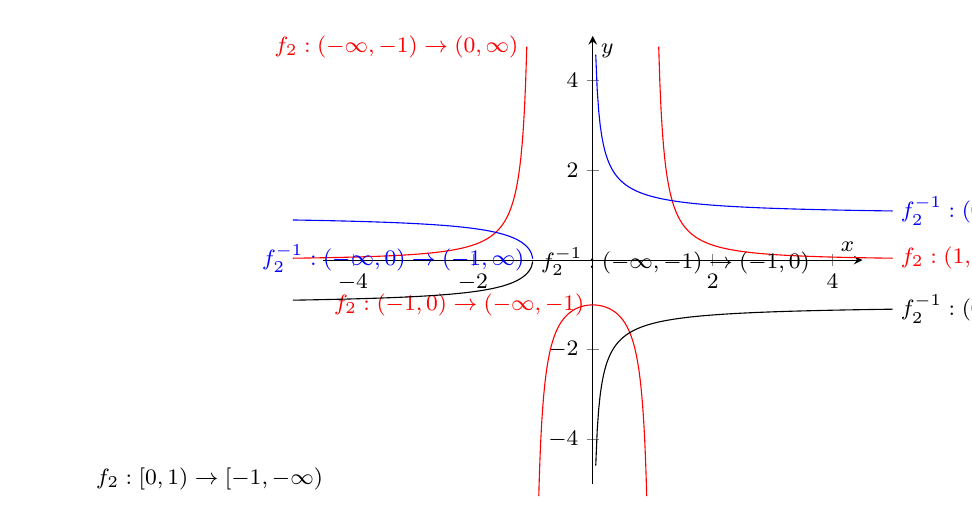
\begin{tikzpicture}
    \begin{axis}[
     axis lines=middle,clip=false,
            xmin=-4.5,xmax=4.5, ymin=-5,ymax=5,
            xticklabel style={black},
            xlabel=$x$,
            ylabel=$y$]
    \addplot[domain=-5:-1.1,samples=200,red]{1/(x^2-1)}
    node[left,pos=1.,font=\footnotesize]{$f_2:(-\infty, -1) \to (0,\infty)$};
    \addplot[domain=-0.9:0,samples=200,red]{1/(x^2-1)}
    node[left,pos=1.,font=\footnotesize]{$f_2:(-1,0) \to (-\infty, -1)$};
    \addplot[domain=0:0.9,samples=200,red]{1/(x^2-1)};
    node[left,pos=1.,font=\footnotesize]{$f_2:[0,1) \to [-1,-\infty)$};
    \addplot[domain=1.1:5,samples=200,red]{1/(x^2-1)}
    node[right,pos=1.,font=\footnotesize]{$f_2:(1,\infty) \to (0,\infty)$};
    \addplot[domain=-5:-1.001,samples=200,blue]{sqrt((1+x)/x)}
    node[left,pos=1.,font=\footnotesize]{$f_2^{-1}:(-\infty,0) \to (-1,\infty)$};
    \addplot[domain=0.05:5,samples=200,blue]{sqrt((1+x)/x)}
    node[right,pos=1.,font=\footnotesize]{$f_2^{-1}:(0,\infty) \to (1,\infty)$};
    \addplot[domain=-5:-1.001,samples=200,black]{-sqrt((1+x)/x)}
    node[right,pos=1.,font=\footnotesize]{$f_2^{-1}:(-\infty,-1) \to (-1,0)$};
    \addplot[domain=0.05:5,samples=200,black]{-sqrt((1+x)/x)}
    node[right,pos=1.,font=\footnotesize]{$f_2^{-1}: (0,\infty) \to (-\infty,-1)$};
    \end{axis}
\end{tikzpicture}
\newpage

\item
Die Funktion $\arcsin(x)$ ist die Umkehrfunktion von $\sin(x)$, wenn nur der Hauptwert betrachtet wird.
Nach Definition, schr\"anken wir den Definitionsbereich von $\sin(x)$ ein auf $-\frac{\pi}{2} \leq x \leq \frac{\pi}{2}$, 
w\"ahrend der Wertebereich $[-1,1]$ ist.
Die erste Ableitung von $\sin(x)$ ist $\cos(x) \geq 0$ f\"ur alle $x \in [-\frac{\pi}{2},\frac{\pi}{2}]$,
daher ist die Funktion monoton steigend und folglich injektiv.
Als Abbildung $f_3 : [-\frac{\pi}{2},\frac{\pi}{2}] \to [-1,1]$ ist die Funktion bijektiv.
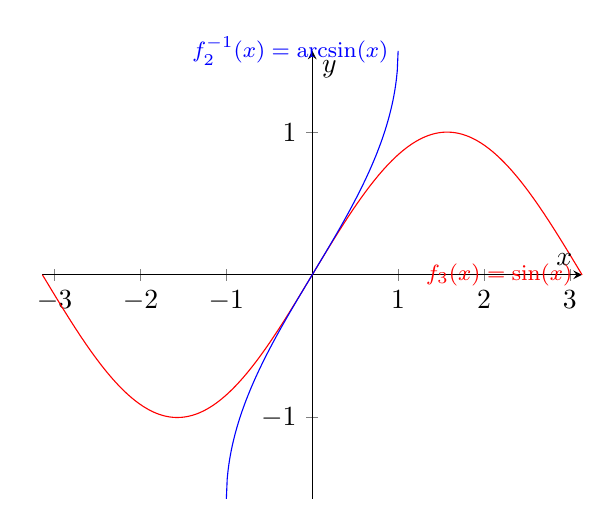
\begin{tikzpicture}
    \begin{axis}[
     axis lines=middle,clip=false,
            xmin=-pi,xmax=pi, ymin=-pi/2,ymax=pi/2,
            xticklabel style={black},
            xlabel=$x$,
            ylabel=$y$]
    \addplot[domain=-pi:pi,samples=200,red]{sin(deg(x))}
    node[left,pos=1.,font=\footnotesize]{$f_3(x)=\sin(x)$};
    \addplot[domain=-1:1,samples=200,blue]{asin(x)/180*pi}
    node[left,pos=1.,font=\footnotesize]{$f_2^{-1}(x)=\arcsin(x)$};
    \end{axis}
\end{tikzpicture}
\newpage
\item
Die Funktion $\arctan(x)$ ist die Umkehrfunktion von $\tan(x)$, wenn nur der Hauptwert betrachtet wird. 
Nach Definition beschr\"anken wir den Definitionsbereich von $\tan(x)$ auf $-\frac{\pi}{2}< x <\frac{\pi}{2}$, 
w\"ahrend der Wertebereich $(-\infty,\infty)$ ist.
Die erste Ableitung von $\tan(x)$ ist $\frac{1}{\cos^2(x)} > 0$ f\"ur alle $x \in (-\frac{\pi}{2},\frac{\pi}{2})$, daher ist die Funktion 
monoton steigend und folglich injektiv. 
Als Abbildung $f_3 : (-\frac{\pi}{2},\frac{\pi}{2}) \to (-\infty,\infty)$ ist sie bijektiv
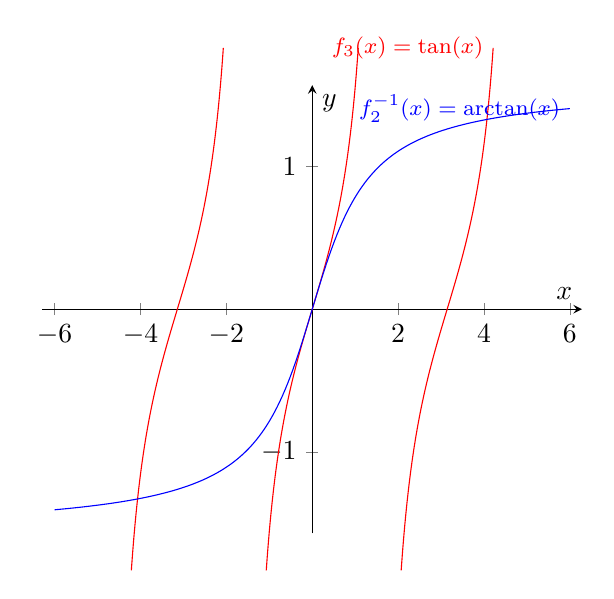
\begin{tikzpicture}
    \begin{axis}[
     axis lines=middle,clip=false,
            xmin=-2*pi,xmax=2*pi, ymin=-pi/2,ymax=pi/2,
            xticklabel style={black},
            xlabel=$x$,
            ylabel=$y$]
    \addplot[domain=-pi/2+0.5:pi/2-0.5,samples=200,red]{tan(deg(x))};
    \addplot[domain=-3*pi/2+0.5:-pi/2-0.5,samples=200,red]{tan(deg(x))};
    \addplot[domain=pi/2+0.5:3*pi/2-0.5,samples=200,red]{tan(deg(x))}
    node[left,pos=1.,font=\footnotesize]{$f_3(x)=\tan(x)$};
    \addplot[domain=-6:6,samples=200,blue]{atan(x)/180*pi}
    node[left,pos=1.,font=\footnotesize]{$f_2^{-1}(x)=\arctan(x)$};
    \end{axis}
\end{tikzpicture}
%clear all
%close all
%
%f=@(x) exp(1./x)
%
%% plot function and inverse branches
%
%% pt. I
%a=-3; b=-.01;
%
%x=linspace(a,b,100)';
%y=f(x);
%
%figure, plot(x,y,'LineWidth',2), hold on, grid, plot(y,x,'LineWidth',2), axis equal
%
%% pt. II
%a=.8; b=3.5;
%
%x=linspace(a,b,100)';
%y=f(x);
%
%figure, plot(x,y,'LineWidth',2), hold on, grid, plot(y,x,'LineWidth',2), axis equal

%clear all
%close all
%
%f=@(x) 1./(x.*x-1)
%
%% plot function and inverse branches
%
%% pt. I
%a=-10; b=-1.1;
%
%x=linspace(a,b,100)';
%y=f(x);
%
%figure, plot(x,y,'LineWidth',2), hold on, grid, plot(y,x,'LineWidth',2), axis equal
%
%% pt. II
%a=-.9; b=-.01;
%
%x=linspace(a,b,100)';
%y=f(x);
%
%figure, plot(x,y,'LineWidth',2), hold on, grid, plot(y,x,'LineWidth',2), axis equal
%
%% pt. III
%a=0; b=.9;
%
%x=linspace(a,b,100)';
%y=f(x);
%
%figure, plot(x,y,'LineWidth',2), hold on, grid, plot(y,x,'LineWidth',2), axis equal
%
%% pt. IV
%a=1.1; b=10;
%
%x=linspace(a,b,100)';
%y=f(x);
%
%figure, plot(x,y,'LineWidth',2), hold on, grid, plot(y,x,'LineWidth',2), axis equal

\end{iii}
}


